\subsection{Dinamično programiranje}

\begin{naloga}{?}{Vaje OR 6.4.2016}
\begin{vprasanje}
Na avtocestni odsek dolžine $M$ kilometrov
želimo postaviti oglasne plakate.
Dovoljene lokacije plakatov določa urad za oglaševanje
in so predstavljene s števili $x_1, x_2, \dots x_n$,
kjer $x_i$ ($1 \le i \le n$)
predstavlja oddaljenost od začetka odseka v kilometrih.
Profitabilnost oglasa na lokaciji $x_i$ določa vrednost $v_i$
($1 \le i \le n$).
Urad za oglaševanje podaja tudi omejitev,
da mora biti razdalja med oglasi vsaj $d$ kilometrov.
Oglase želimo postaviti tako, da bodo čim bolj profitabilni.
\begin{enumerate}[(a)]
\item Reši problem za parametre $M = 20$, $d = 5$, $n = 8$,
$(x_i)_{i=1}^n = (1, 2, 8, 10, 12,$ $14, 17, 20)$ in
$(v_i)_{i=1}^n = (8, 8, 12, 10, 7, 5, 6, 10)$.
\item Napiši rekurzivne enačbe za opisani problem.
\item Napiši algoritem,
ki poišče najbolj profitabilno postavitev oglasov za dane parametre.
Kakšna je njegova časovna zahtevnost?
\end{enumerate}

\end{vprasanje}
\begin{odgovor}
\end{odgovor}
\end{naloga}


\begin{naloga}{?}{Vaje OR 6.4.2016}
\begin{vprasanje}
Imamo nahrbtnik nosilnosti $M$ kilogramov.
Danih je $n$ objektov z vrednostmi $v_i$ in težami $t_i$ ($1 \le i \le n$).
Problem nahrbtnika sprašuje po izbiri predmetov
$I \subseteq \{1, 2, \dots, n\}$,
ki maksimizira njihovo skupno vrednost pri omejitvi $\sum_{i \in I} t_i \le M$.
\begin{enumerate}[(a)]
\item Napiši rekurzivne enačbe za opisani problem.
\item Z uporabo rekurzivnih enačb reši problem za parametre $M = 8$, $n = 8$,
$(v_i)_{i=1}^n = (9, 9, 8, 11, 10, 15,$ $3, 12)$ in
$(t_i)_{i=1}^n = (3, 5, 1, 4, 3, 8, 2, 7)$.
\end{enumerate}

\end{vprasanje}
\begin{odgovor}
\end{odgovor}
\end{naloga}


\begin{naloga}{?}{Vaje OR 6.4.2016}
\begin{vprasanje}
Dana je matrika $A = (a_{ij})_{i,j=1}^{m,n}$.
Poiskati želimo pot minimalne vsote,
ki se začne v levem zgornjem kotu (pri $a_{11}$)
in konča v desnem spodnjem kotu (pri $a_{mn}$).
Dovoljeni so zgolj premiki v desno in navzdol.
\begin{enumerate}[(a)]
\item Reši problem za matriko
$$
A = \begin{pmatrix}
131 & 673 & 234 & 103 &  18 \\
201 &  96 & 342 & 965 & 150 \\
630 & 803 & 746 & 422 & 111 \\
537 & 699 & 497 & 121 & 956 \\
805 & 732 & 524 &  37 & 332
\end{pmatrix} .
$$
\item Napiši rekurzivne enačbe za opisani problem.
\item Na osnovi rekurzivnih enačb napiši algoritem, ki reši opisani problem.
Oceni tudi njegovo časovno zahtevnost v odvisnosti od $m$ in $n$.
\end{enumerate}

\end{vprasanje}
\begin{odgovor}
\end{odgovor}
\end{naloga}


\begin{naloga}{?}{Vaje OR 6.4.2016}
\begin{vprasanje}
Dan je niz $S = a_1 a_2 \dots a_n$,
kjer so $a_i$ ($1 \le i \le n$) elementi neke končne abecede.
Nizu $a_j a_{j+1} \dots a_k$, kjer je $1 \le j \le k \le n$,
pravimo {\em strnjen podniz} niza $S$.
S pomočjo dinamičnega programiranja napiši algoritem,
ki določi najdaljši palindromski strnjen podniz v $S$.

\end{vprasanje}
\begin{odgovor}
\end{odgovor}
\end{naloga}


\begin{naloga}{?}{Vaje OR 6.4.2016}
\begin{vprasanje}
Dana je matrika $A = (a_{ij})_{i,j=1}^{m,n}$.
Poiskati želimo strnjeno podmatriko matrike $A$
z največjo vsoto komponent.
\begin{enumerate}[(a)]
\item Reši problem za matriko
$$
A = \begin{pmatrix}
 1 & -1 &  2 &  4 \\
-3 & -2 &  8 &  2 \\
-3 &  2 & -2 &  4 \\
 1 & -5 & -1 & -2
\end{pmatrix} .
$$
\item Napiši rekurzivne enačbe za opisani problem.
\item Napiši algoritem, ki reši opisani problem.
Oceni tudi njegovo časovno zahtevnost v odvisnosti od $m$ in $n$.
\end{enumerate}

\end{vprasanje}
\begin{odgovor}
\end{odgovor}
\end{naloga}


\begin{naloga}{?}{Vaje OR 6.4.2016}
\begin{vprasanje}
Na voljo imamo kovance z vrednostmi $1 = v_1 < v_2 < \cdots < v_n$
in vsoto $C$, ki jo želimo izplačati s kovanci.
Predpostavljamo, da imamo dovolj velik nabor kovancev.
\begin{enumerate}[(a)]
\item Poišči izplačilo z najmanjšim številom kovancev
za $C = 25$, $n = 4$ in $(v_i)_{i=1}^n = (1, 2, 5, 7)$.
\item S pomočjo dinamičnega programiranja reši problem v splošnem.
\end{enumerate}

\end{vprasanje}
\begin{odgovor}
\end{odgovor}
\end{naloga}


\begin{naloga}{?}{Vaje OR 6.4.2016}
\begin{vprasanje}
Na ulici je $n$ vrstnih hiš,
pri čemer je v $i$-ti hiši $c_i$ denarja.
Tat se odloča, katere izmed hiš naj oropa.
Vsak oropan stanovalec to sporoči svojim sosedom,
zato tat ne sme oropati dveh sosednjih hiš.
Ker je tat poslušal predmet Operacijske raziskave,
pozna dinamično programiranje.
Pokaži, kako naj tat določi, katere hiše naj oropa.

\end{vprasanje}
\begin{odgovor}
\end{odgovor}
\end{naloga}


\begin{naloga}{?}{Kolokvij OR 31.5.2012}
\begin{vprasanje}
Imamo hlod dolžine $\ell$,
ki bi ga radi razžagali na $n$ označenih mestih
$0 < x_1 < x_2 < \dots < x_n < \ell$.
Eno rezanje stane toliko, kolikor je dolžina hloda, ki ga režemo.
Ko hlod prerežemo, dobimo dva manjša hloda, ki ju režemo naprej.
Poiskati želimo zaporedje rezanj z najmanjšo ceno.
\begin{enumerate}[(a)]
\item Reši problem pri podatkih $\ell = 10$ in $(x)_{i=1}^4 = (3, 5, 7, 8)$.
\item S pomočjo dinamičnega programiranja reši problem v splošnem.
Oceni tudi njegovo časovno zahtevnost.
\end{enumerate}

\end{vprasanje}
\begin{odgovor}
\end{odgovor}
\end{naloga}


\begin{naloga}{Hillier, Lieberman}{\cite[Problem~11.3-1]{hl}}
\begin{vprasanje}
Lastnik verige $n$ trgovin z živili je kupil $m$ zabojev svežih jagod.
Naj bo $p_{ij}$ pričakovan dobiček v trgovini $j$,
če tja dostavimo $i$ zabojev.
Zanima nas, koliko zabojev naj gre v vsako trgovino,
da bomo imeli čim večji zaslužek.
Zaradi logističnih razlogov zabojev ne želimo deliti.
\begin{enumerate}[(a)]
\item Z dinamičnim programiranjem reši problem za podatke $m = 5$, $n = 3$
in $p_{ij}$ iz sledeče tabele:
$$
\begin{array}{c|ccc}
p_{ij} & 1 & 2 & 3 \\
\hline
0 &  0 &  0 &  0 \\
1 &  5 &  6 &  4 \\
2 &  9 & 11 &  9 \\
3 & 14 & 15 & 13 \\
4 & 17 & 19 & 18 \\
5 & 21 & 22 & 20 \\
\end{array}
$$
\item Napiši algoritem, ki reši opisani problem v splošnem.
\end{enumerate}

\end{vprasanje}
\begin{odgovor}
\end{odgovor}
\end{naloga}


\begin{naloga}{Hillier, Lieberman}{\cite[Problem~11.3-8]{hl}}
\begin{vprasanje}
Podjetje bo kmalu uvedlo nov izdelek na zelo konkurenčen trg,
zato trenutno pripravlja marketinško strategijo.
Odločili so se, da bodo izdelek uvedli v treh fazah.
V prvi fazi bodo pripravili posebno začetno ponudbo z močno znižano ceno,
da bi privabili zgodnje kupce.
Druga faza bo vključevala intenzivno oglaševalsko kampanjo,
da bi zgodnje kupce prepričali, naj izdelek še vedno kupujejo po redni ceni.
Znano je, da bo ob koncu druge faze
konkurenčno podjetje predstavilo svoj izdelek.
Zato bo v tretji fazi okrepljeno oglaševanje z namenom,
da bi preprečili beg strank h konkurenci.

Podjetje ima za oglaševanje na voljo $4$ milijone evrov,
ki jih želimo čim bolj učinkovito porabiti.
Naj bo $m$ tržni delež v procentih, pridobljen v prvi fazi,
$f_2$ delež, ohranjen po drugi fazi,
in $f_3$ delež, ohranjen po tretji fazi.
Maksimizirati želimo končni tržni delež, torej količino $m f_2 f_3$.

\begin{enumerate}[(a)]
\item Denimo, da želimo v vsaki fazi porabiti nek večkratnik milijona evrov,
pri čemer bomo pri prvi fazi porabili vsaj milijon evrov.
V spodnji tabeli so zbrani vplivi porabljenih količin
na vrednosti $m$, $f_2$ in $f_3$.
$$
\begin{array}{c|ccc}
M€ & m & f_2 & f_3 \\
\hline
0 &  - & 0.2 & 0.3 \\
1 & 20 & 0.4 & 0.5 \\
2 & 30 & 0.5 & 0.6 \\
3 & 40 & 0.6 & 0.7 \\
4 & 50 &   - &   - \\
\end{array}
$$
Kako naj razdelimo sredstva?
\item Denimo sedaj,
da lahko v vsaki fazi porabimo poljubno pozitivno količino denarja
(seveda glede na omejitev skupne porabe).
Naj bodo torej $x_1$, $x_2$ in $x_3$ količine denarja v milijonih evrov,
ki jih porabimo v prvi, drugi in tretji fazi.
Vpliv na tržni delež je podan s formulami
$$
m = x_1 (10 - x_1), \quad
f_2 = 0.4 + 0.1 x_2, \quad \text{in} \quad
f_3 = 0.6 + 0.07 x_3 .
$$
Kako naj sedaj razdelimo sredstva?
\end{enumerate}

\end{vprasanje}
\begin{odgovor}
\end{odgovor}
\end{naloga}


\begin{naloga}{?}{Izpit OR 26.6.2012}
\begin{vprasanje}
Nori profesor Boltežar stanuje v stolpnici z $n$ nadstropji,
oštevilčenimi od $1$ do $n$.
Nori stanovalci tega bloka radi mečejo cvetlične lončke z balkonov.
Boltežar bi rad ugotovil, katero je najvišje nadstropje,
s katerega lahko pade cvetlični lonček, ne da bi se razbil.
Jasno je, da če se lonček razbije pri padcu iz $k$-tega nadstropja,
potem se razbije tudi pri padcu s $(k+1)$-tega nadstropja.
Če bi Boltežar imel le en cvetlični lonček,
bi ga lahko metal po vrsti od najnižjega nadstropja navzgor,
dokler se ne bi razbil.
V najslabšem primeru bi lonček torej vrgel $n$ krat
(možno je, da bi lonček preživel tudi padec iz najvišjega nadstropja).

Ker ima Boltežar doma $k$ cvetličnih lončkov,
lahko do rezultata pride tudi z manjšim številom metov.
S pomočjo dinamičnega programiranja bi rad poiskal strategijo metanja,
ki bi minimizirala število potrebnih metov v najslabšem primeru.
\begin{enumerate}[(a)]
\item Napiši rekurzivne enačbe za opisani problem.
\item Napiši algoritem, ki reši opisani problem.
Oceni tudi njegovo časovno zahtevnost v odvisnosti od $n$ in $k$.
\end{enumerate}

\end{vprasanje}
\begin{odgovor}
\end{odgovor}
\end{naloga}


\begin{naloga}{Hillier, Lieberman}{\cite[Problem~11.2-2]{hl}}
\begin{vprasanje}
Vodja prodaje pri založniku učbenikov za fakulteto
ima na voljo $6$ trgovskih potnikov,
ki jim želi dodeliti eno od treh regij, v kateri bodo delovali.
V vsaki regiji mora delovati vsaj en trgovski potnik.
Naj bo $p_{ij}$ pričakovana porast v prodaji v regiji $j$,
če bo tam delovalo $i$ trgovskih potnikov:
$$
\begin{array}{c|ccc}
p_{ij} & 1 & 2 & 3 \\
\hline
1 & 35 & 21 & 28 \\
2 & 48 & 42 & 41 \\
3 & 70 & 56 & 63 \\
4 & 89 & 70 & 75 \\
\end{array}
$$
Reši problem s pomočjo dinamičnega programiranja.

\end{vprasanje}
\begin{odgovor}
\end{odgovor}
\end{naloga}


\begin{naloga}{Hillier, Lieberman}{\cite[Problem~11.3-16]{hl}}
\begin{vprasanje}
Dan je sledeči nelinearni program.
\begin{align*}
\max &\quad 2x_1^2 + 2x_2 + 4x_3 - x_3^2 \\[1ex]
2x_1 + x_2 + x_3 &\le 4 \\
x_1, x_2, x_3 &\ge 0
\end{align*}
Reši ga s pomočjo dinamičnega programiranja.

\end{vprasanje}
\begin{odgovor}
\end{odgovor}
\end{naloga}


\begin{naloga}{Hillier, Lieberman}{\cite[Problem~11.4-1]{hl}}
\begin{vprasanje}
Igralec na srečo bo odigral tri partije s svojimi prijatelji,
pri čemer lahko vsakič stavi na svojo zmago.
Stavi lahko katerokoli vsoto denarja, ki jo ima na voljo
-- če izgubi partijo, zastavljeno vsoto izgubi, sicer pa tako vsoto pridobi.
Pri vsaki partiji sta verjetnosti zmage in poraza enaki $1/2$.
Na začetku ima $75 €$, na koncu pa želi imeti $100 €$
(ker igra s prijatelji, noče imeti več kot toliko).

Z dinamičnim programiranjem poišči strategijo stavljenja,
ki maksimizira verjetnost, da bo na koncu imel natanko $100 €$.
\end{vprasanje}
\begin{odgovor}
\end{odgovor}
\end{naloga}


\begin{naloga}%
{Dasgupta, Papadimitriou, Vazirani}{\cite[Exercise~6.14]{dpv}}
\begin{vprasanje}[nal:blago]
Imamo pravokoten kos blaga dimenzij $m \times n$,
kjer sta $m$ in $n$ pozitivni celi števili,
ter seznam $k$ izdelkov,
pri čemer potrebujemo za izdelek $i$
pravokoten kos blaga dimenzij $a_i \times b_i$
($a_i, b_i$ sta pozitivni celi števili),
ki ga prodamo za ceno $c_i > 0$.
Imamo stroj, ki lahko poljuben kos blaga razreže na dva dela
bodisi vodoravno, bodisi navpično.
Začetni kos blaga želimo razrezati tako,
da bomo lahko naredili izdelke,
ki nam bodo prinašali čim večji dobiček.
Pri tem smemo izdelati poljubno število kosov posameznega izdelka.
Kose blaga lahko seveda tudi obračamo
(tj., za izdelek $i$ lahko narežemo kos velikosti
$a_i \times b_i$ ali $b_i \times a_i$).

Zapiši rekurzivne enačbe za reševanje danega problema.
Razloži, kaj predstavljajo spremenljivke,
v kakšnem vrstnem redu jih računamo,
ter kako dobimo optimalno rešitev.
\end{vprasanje}
\begin{odgovor}
\end{odgovor}
\end{naloga}


\begin{naloga}{Janoš Vidali}{Izpit OR 15.12.2016}
\begin{vprasanje}
Oceni časovno zahtevnost algoritma,
ki sledi iz rekurzivnih enačb za nalogo~\ref{nal:blago}.
Reši problem za podatke $m = 5, n = 3, k = 4$,
$(a_i)_{i=1}^k = (2, 3, 1, 2)$, $(b_i)_{i=1}^k = (2, 1, 4, 3)$
in $(c_i)_{i=1}^k = (6, 3, 5, 7)$.
\end{vprasanje}
\begin{odgovor}
\end{odgovor}
\end{naloga}


\begin{naloga}{Janoš Vidali}{Izpit OR 31.1.2017}
\begin{vprasanje}
Dano je zaporedje $n$ realnih števil $a_1, a_2, \dots, a_n$.
Želimo poiskati strnjeno podzaporedje z največjim produktom
-- t.j., taka indeksa $i, j$ ($1 \le i \le j \le n$),
da je produkt $a_i a_{i+1} \cdots a_{j-1} a_j$ čim večji.

\begin{enumerate}[(a)]
\item Zapiši rekurzivne enačbe za reševanje danega problema.
Razloži, kaj predstavljajo spremenljivke,
v kakšnem vrstnem redu jih računamo,
ter kako dobimo optimalno rešitev. \\
{\small {\bf Namig:}
posebej obravnavaj pozitivne in negativne delne produkte.}

\item Oceni časovno zahtevnost algoritma, ki sledi iz zgoraj zapisanih enačb.

\item S svojim algoritmom reši problem za zaporedje
$$
0.9, \ -2, \ -0.6, \ -0.5, \ -2, \ 5, \ 0.1, \ 3, \ 0.5, \ -3 \ .
$$
\end{enumerate}
\end{vprasanje}
\begin{odgovor}
\end{odgovor}
\end{naloga}


\begin{naloga}{Sergio Cabello}{Izpit OR 15.3.2017}
\begin{vprasanje}
Za zaporedje števil $x_1, x_2, \dots x_m$ pravimo, da je {\em oscilirajoče},
če velja $x_i < x_{i+1}$ za vse sode $i$ in $x_i > x_{i+1}$ za vse lihe $i$.
S pomočjo dinamičnega programiranja zasnuj algoritem,
ki v polinomskem času izračuna dolžino najdaljšega oscilirajočega podzaporedja
zaporedja celih števil $a_1, a_2, \dots a_n$.
\end{vprasanje}
\begin{odgovor}
\end{odgovor}
\end{naloga}


\begin{naloga}{Janoš Vidali}{Izpit OR 10.7.2017}
\begin{vprasanje}
V podjetju imajo na voljo $m$ milijonov evrov sredstev,
ki jih bodo vložili v razvoj nove aplikacije.
Denar bodo porazdelili med tri skupine.
Naj bodo $x_1$, $x_2$ in $x_3$ količine denarja (v milijonih evrov),
ki jih bodo dodelili razvijalcem, oblikovalcem in marketingu.
Vrednosti $x_1, x_2, x_3$ niso nujno cela števila.
Razvijalci morajo dobiti vsaj $a_1$ milijonov evrov,
potencial, ki ga ustvarijo, pa je $p_1 = n_1 + k_1 x_1$.
Oblikovalci morajo dobiti vsaj $a_2$ milijonov evrov,
potencial, ki ga ustvarijo, pa je $p_2 = n_2 + k_2 x_2$.
Marketing mora dobiti vsaj $a_3$ milijonov evrov,
ustvari pa faktor $p_3 = n_3 + k_3 x_3$.
Pričakovani dobiček v milijonih evrov
se izračuna po formuli $d = (p_1 + p_2) p_3$.
V podjetju bi radi sredstva porazdelili med skupine tako,
da bo pričakovani dobiček čim večji.

\begin{enumerate}[(a)]
\item Zapiši rekurzivne enačbe za reševanje danega problema.
\item Z zgoraj zapisanimi enačbami reši problem
pri podatkih $m = 15$, $a_1 = 4$, $n_1 = 3$, $k_1 = 1.5$,
$a_2 = 3$, $n_2 = 4$, $k_2 = 2$, $a_3 = 2$, $n_3 = 0.4$ in $k_3 = 0.3$.
\end{enumerate}
\end{vprasanje}
\begin{odgovor}
\end{odgovor}
\end{naloga}


\begin{naloga}{Janoš Vidali}{Izpit OR 29.8.2017}
\begin{vprasanje}
V veliki multinacionalni korporaciji želijo,
da bi se zakonodaja spremenila v njihov prid.
V ta namen so najeli $m$ lobistov,
ki se bodo pogajali z $n$ političnimi strankami,
da pridobijo njihovo podporo pri spremembi zakonodaje.
Vsak lobist se bo pogajal s samo eno stranko;
k vsaki stranki lahko pošljejo več lobistov.
Naj bo $p_{ij}$ ($0 \le i \le m$, $1 \le j \le n$) verjetnost,
da pridobijo podporo stranke $j$,
če se z njo pogaja $i$ lobistov
(lahko predpostaviš $p_{i-1,j} \le p_{ij}$ za vsaka $i, j$).
Verjetnosti za različne stranke so med seboj neodvisne.
Maksimizirati želijo verjetnost,
da bodo lobisti pridobili podporo vseh $n$ političnih strank.

\begin{enumerate}[(a)]
\item Zapiši rekurzivne enačbe za reševanje danega problema.
\item Naj bo $m = 6$ in $n = 3$.
K vsaki stranki želijo poslati vsaj enega lobista
(tj., $p_{0j} = 0$ za vsak $j$),
vrednosti $p_{ij}$ za $i \ge 1$ pa so podane v spodnji tabeli.
$$
\begin{array}{c|ccc}
p_{ij} & 1 & 2 & 3 \\ \hline
1 & 0.2 & 0.4 & 0.3 \\
2 & 0.5 & 0.5 & 0.4 \\
3 & 0.7 & 0.5 & 0.8 \\
4 & 0.8 & 0.6 & 0.9 \\
\end{array}
$$
Za dane podatke reši problem z zgoraj zapisanimi enačbami.
\end{enumerate}
\end{vprasanje}
\begin{odgovor}
\end{odgovor}
\end{naloga}


\begin{naloga}{Janoš Vidali}{Kolokvij OR 23.4.2018}
\begin{vprasanje}[nal:domine]
Imamo zaporedje $n$ polj,
pri čemer je na $i$-tem polju zapisano število $a_i$.
Na voljo imamo še $\lfloor n/2 \rfloor$ domin,
z vsako od katerih lahko pokrijemo dve sosednji polji.
Vsaka domina je sestavljena iz dveh delov:
na enem je znak $+$, na drugem pa znak $-$.
Posamezno polje lahko pokrijemo z le eno domino;
če sta pokriti dve sosednji polji, morata biti pokriti z različnima znakoma
(bodisi z iste, bodisi z druge domine).
Iščemo tako postavitev domin,
ki maksimizira vsoto pokritih števil,
pomnoženih z znakom na delu domine, ki pokriva število.
Pri tem ni potrebno, da uporabimo vse domine.
Primer je podan na sliki~\ref{fig:domine}.

\begin{enumerate}[(a)]
\item Zapiši rekurzivne enačbe za reševanje danega problema.
Razloži, kaj predstavljajo spremenljivke,
v kakšnem vrstnem redu jih računamo,
ter kako dobimo optimalno rešitev. \\
{\small {\bf Namig:}
posebej obravnavaj dva primera glede na postavitev zadnje domine.}

\item Oceni časovno zahtevnost algoritma, ki sledi iz zgoraj zapisanih enačb.

\item S svojim algoritmom poišči optimalno pokritje
za primer s slike~\ref{fig:domine}.
\end{enumerate}

\begin{figure}
\centering
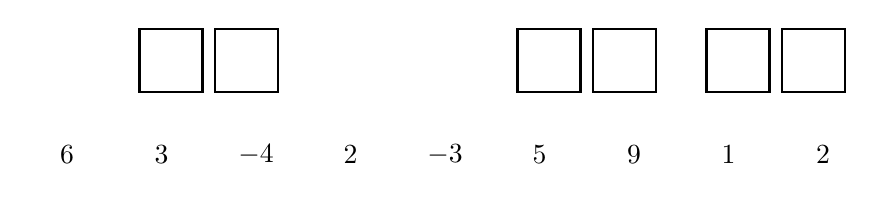
\begin{tikzpicture}[style=thick,scale=1.2]
\tikzstyle{field}=[rectangle, minimum size=10mm]
\tikzstyle{domino}=[field, draw, minimum size=8mm]

\node[field] at (0, 0) {$6$};
\node[field] at (1, 0) {$3$};
\node[field] at (2, 0) {$-4$};
\node[field] at (3, 0) {$2$};
\node[field] at (4, 0) {$-3$};
\node[field] at (5, 0) {$5$};
\node[field] at (6, 0) {$9$};
\node[field] at (7, 0) {$1$};
\node[field] at (8, 0) {$2$};

\node[domino] at (1.1, 1) {$\pp$};
\node[domino] at (1.9, 1) {$\mm$};
\node[domino] at (5.1, 1) {$\mm$};
\node[domino] at (5.9, 1) {$\pp$};
\node[domino] at (7.1, 1) {$\mm$};
\node[domino] at (7.9, 1) {$\pp$};
\end{tikzpicture}
\caption{Primer dopustnega (ne nujno optimalnega) pokritja
za nalogo~\ref{nal:domine}.
Vsota tega pokritja je $3 - (-4) - 5 + 9 - 1 + 2 = 12$.
Če bi eno od zadnjih dveh domin obrnili (zamenjala bi se znaka),
dobljeno pokritje ne bi bilo dopustno,
saj bi dve zaporedni polji bili pokriti z enakima znakoma.}
\label{fig:domine}
\end{figure}
\end{vprasanje}
\begin{odgovor}
\end{odgovor}
\end{naloga}


\begin{naloga}{Janoš Vidali}{Izpit OR 5.7.2018}
\begin{vprasanje}
Vlagatelj ima na voljo $50$ milijonov evrov sredstev,
ki jih lahko porabi za donosno, a tvegano naložbo.
Ocenjuje, da bi se mu ob uspehu naložbe vložek povrnil petkratno,
verjetnost uspeha pa ocenjuje na $0.6$.
Zaradi tveganja se lahko odloči za zavarovanje naložbe,
pri čemer ima ponudbi dveh zavarovalnic,
ki mu proti plačilu ustrezne premije ponujata povračilo dela vložka,
če bo naložba neuspešna.
Vlagatelj lahko del sredstev obdrži tudi zase
(tj., ga ne porabi za naložbo ali premijo).

Naj bodo torej $x_1, x_2, x_3$ vrednosti v milijonih evrov,
ki zaporedoma predstavljajo količine,
ki jih vlagatelj obrži zase, porabi za naložbo,
in plača za zavarovalniško premijo.
Pričakovana vrednost naložbene strategije vlagatelja
(tj., količina denarja, ki jo ima na koncu)
je potem
$$
x_1 + x_2 (0.6 \cdot 5 + 0.4 q(x_3)) ,
$$
kjer $q(x_3)$ predstavlja delež vložka,
ki ga glede na vloženo premijo zavarovalnica povrne ob ne\-uspe\-hu naložbe.

Vlagatelj ima dve ponudbi konkurenčnih zavarovalnic.
Zavarovalnica Zvezna d.z.z.~za premijo v višini $x_3$ milijonov evrov
ponuja povračilo deleža $0.15 x_3$ celotne naložbe v primeru neuspeha,
pri čemer je največja možna premija $4$ milijone evrov.
Zavarovalnica Diskretna d.d.z.~pa ponuja le tri možne premije:
\begin{center}
\begin{tabular}{c|c}
premija & delež povračila ob neuspešni naložbi \\ \hline
$1$ milijon evrov & $0.1$ \\
$2$ milijona evrov & $0.35$ \\
$3$ milijoni evrov & $0.5$
\end{tabular}
\end{center}
Pogodbo smemo skleniti samo pri eni zavarovalnici.

\begin{enumerate}[(a)]
\item Zapiši definicijo funkcije $q(x)$
skupaj z izbiro najugodnejše zavarovalnice pri vsakem $x$.

\item Zapiši rekurzivne formule za določitev strategije vlaganja,
ki nam bo prinesla največji pričakovani dobiček.

\item S pomočjo zgornjih rekurzivnih enačb ugotovi,
kako naj ravna vlagatelj, da bo imel čim večji dobiček.
\end{enumerate}
\end{vprasanje}
\begin{odgovor}
\end{odgovor}
\end{naloga}


\begin{naloga}{Janoš Vidali}{Izpit OR 28.8.2018}
\begin{vprasanje}
Pri direkciji za ceste načrtujejo nov avtocestni odsek dolžine $M$ kilometrov.
Ob cesti želijo zgraditi počivališča tako,
da je razdalja med dvema zaporednima počivališčema največ $K$ kilometrov.
Prav tako mora biti prvo počivališče največ $K$ kilometrov od začetka,
zadnje pa največ $K$ kilometrov od konca avtocestnega odseka.
Naj bodo $x_1 < x_2 < \dots < x_n$ možne lokacije počivališč
(v kilometrih od začetka avtocestnega odseka),
in $c_i$ ($1 \le i \le n$) cena izgradnje počivališča na lokaciji $x_i$.
Postavitev počivališč želijo izbrati tako,
da bo skupna cena izgradnje čim manjša.

\begin{enumerate}[(a)]
\item Zapiši rekurzivne enačbe za reševanje danega problema.
Razloži, kaj predstavljajo spremenljivke,
v kakšnem vrstnem redu jih računamo, ter kako dobimo optimalno rešitev.

\item Oceni časovno zahtevnost algoritma, ki sledi iz zgoraj zapisanih enačb.

\item S pomočjo rekurzivnih enačb reši zgornji problem za podatke
\begin{align*}
M &= 100, & (x_i)_{i=1}^8 &= ( 5, 12, 22, 34, 49, 65, 83, 91), \\
K &= 30,  & (c_i)_{i=1}^8 &= (18, 11, 21, 16, 23, 15, 19, 13).
\end{align*}
\end{enumerate}
\end{vprasanje}
\begin{odgovor}
\end{odgovor}
\end{naloga}
